\documentclass[italian,12pt]{article}

\def\Title{Verbale interno}
\def\Subtitle{Riunione interna settimanale}
\def\Author{7Last}
\def\Date{2024-05-22}
\def\Version{v1.0}

%pacchetti extra da scaricare dblfloatfix, fancyhdr
\usepackage[left=2cm, right=2cm, bottom=3cm, top=3cm]{geometry}
\usepackage{fancyhdr}%creazione header-footer
\usepackage{graphicx} %serve per inserire immagini
\graphicspath{ {../../../logo/} }
%\usepackage{dblfloatfix} %serve per posizionare gli elementi dove si vuole
\usepackage[hidelinks]{hyperref} %serve per i link
\usepackage{tikz}
\usepackage{tgadventor} % font
\usepackage[useregional=numeric,showseconds=true,showzone=false]{datetime2}
\usepackage{caption}

\usepackage{hyperref}
\usepackage{tocloft}
\usepackage{titlesec}
\usepackage{color}
\usepackage{ulem}
\usepackage{pgfplots}
\usepackage{pgf-pie}
\usepackage[italian]{babel}
\usepackage{comment}
\usepackage{tabularx}
\usepackage{longtable}
\usepackage{float}
\usepackage{amsmath}

\linespread{1.2}
\captionsetup[table]{name=Tabella}
\geometry{headsep=1.5cm}

\renewcommand{\contentsname}{Indice}
\renewcommand\familydefault{\sfdefault}
\renewcommand{\listtablename}{Indice delle tabelle}
\renewcommand\familydefault{\sfdefault}
\renewcommand{\listfigurename}{Indice delle immagini}
\renewcommand\familydefault{\sfdefault}

% set sfdefault for page numbers
\let\oldthepage\thepage
\renewcommand{\thepage}{\sffamily\oldthepage}

\begin{document}
\newgeometry{left=2cm,right=2cm,bottom=2.1cm,top=2.1cm}
\begin{titlepage}
    \vspace*{.5cm}

    \vspace{2cm}
    {
        \centering
        {\bfseries\huge \Title\par}
        \bigbreak
        {\bfseries\large \Author\par}
        \bigbreak
        {\Version\par}
        \vfill

        \begin{tikzpicture}[remember picture,overlay]

            \fill[blue!20!black] (current page.south west) -- ++(10cm,0) -- ++(-10cm,15cm) -- cycle;
            \fill[orange] (current page.south east) -- ++(-18cm,0) -- ++(21.6cm,22cm) -- cycle;

            \clip (0,-3cm) circle (2.5cm) node (current page.center) {
\includegraphics[width=5cm]{logo.jpg}};
        \end{tikzpicture}

    }

    \vfill

\end{titlepage}

\restoregeometry





















\newpage
%---------------header------------------%
\pagestyle{fancy}
\fancyhead{} % pulizia degli header
\lhead{%
\begin{tikzpicture}
    \clip (0,0) circle (0.5cm);
    \node at (0,0) {
\includegraphics[width=1cm]{logo}};
\end{tikzpicture}%
}
\chead{\vspace{\fill}\Title\vspace{\fill}}
\rhead{\vspace{\fill}\Version\vspace{\fill}}
%quad è una spaziatura
%---------------------------------------%

\begin{table}[!h]
	\caption*{Versioni}
	\begin{center}
		\begin{tabular}{ c c c c p{6.1cm} }
			\hline                                                                                                 \\[-2ex]
			Ver. & Data       & Redattore          & Verificatore      & Descrizione                                    \\
			\\[-2ex] \hline \\[-1.5ex]
			0.1  & 2024-05-08 & Valerio Occhinegro &                   & Prima Stesura \\
			\\[-1.5ex] \hline
		\end{tabular}
	\end{center}
\end{table}

\newpage
\tableofcontents
\listoftables
\listoffigures
\newpage

\section{Introduzione}
\subsection{Obiettivo del documento}
Il presente documento ha lo scopo di definire le strategie di verifica e validazione utilizzate per assicurare il corretto funzionamento dello strumento sviluppato e delle
attività che lo accompagnano.  Sarà sottoposto a revisioni continue, così da prevedere situazioni precedentemente non occorse e da seguire l'evoluzione del progetto.
\subsection{Glossario}
Il \href{https://7last.github.io/docs/rtb/documentazione-interna/glossario#glossario}{glossario\textsubscript{G}} è uno strumento utilizzato per risolvere eventuali dubbi riguardanti 
alcuni termini specifici utilizzati nella redazione del documento.
Esso conterrà la definizione dei termini evidenziati e sarà consultabile al seguente \href{https://7last.github.io/docs/rtb/documentazione-interna/glossario}{link}. I termini presenti in tale documento saranno evidenziati da una 'G' a pedice.
\subsection{Riferimenti}
\subsubsection{Riferimenti normativi}
\begin{itemize}
    \item \href{https://7last.github.io/docs/rtb/documentazione-interna/glossario#norme-di-progetto}{Norme di progetto\textsubscript{G}} (aggiungere versione e/o link al documento);
    \item Regolamento del progetto:\\
		  \url{https://www.math.unipd.it/~tullio/IS-1/2023/Dispense/PD2.pdf}.
\end{itemize}
\subsubsection{Riferimenti informativi}
\begin{itemize}
    \item \href{https://7last.github.io/docs/rtb/documentazione-interna/glossario#capitolato}{Capitolato\textsubscript{G}} d'appalto C6: \href{https://7last.github.io/docs/rtb/documentazione-interna/glossario#synccity}{SyncCity\textsubscript{G}} – A \href{https://7last.github.io/docs/rtb/documentazione-interna/glossario#smart-city}{smart city\textsubscript{G}} monitoring platform\\
    \url{https://www.math.unipd.it/~tullio/IS-1/2023/Progetto/C6.pdf};
    \item \href{https://it.wikipedia.org/wiki/ISO/IEC_9126}{Standard ISO/IEC 9126};
    \item \href{https://iso25000.com/index.php/en/iso-25000-standards/iso-25010}{Standard ISO/IEC 25010};
    \item \href{ https://en.wikipedia.org/wiki/ISO/IEC_12207}{Standard ISO/IEC 12207:1995};
    \item \href{URL}{\textit{Verbali esterni}};
    \item \href{URL}{\textit{Verbali interni}};
    \item \href{URL}{\href{https://7last.github.io/docs/rtb/documentazione-interna/glossario#analisi-dei-requisiti}{\textit{Analisi dei requisiti}\textsubscript{G}}};
    \item AGGIUNGERE LINK
\end{itemize}

\section{Requisiti}
\subsection{Definizione di un requisito}
Per ciascun requisito vengono fornite le seguenti informazioni:
\begin{itemize}
	\item \textbf{Codice}: codice identificativo del requisito, meglio specificato nella sezione \ref{sec:codifica_requisiti};
	\item \textbf{Descrizione}: breve descrizione del requisito;
	\item \textbf{Fonte}: provenienza del requisito, meglio specificata nella sezione \ref{sec:fonti_requisiti};
	\item \textbf{Importanza}: indica l'importanza del requisito, meglio specificata nella sezione \ref{sec:importanza_requisiti}.
\end{itemize}

\subsection{Tipologie di requisiti}
I requisiti possono essere di quattro tipologie:
\begin{itemize}
	\item \textbf{Funzionali}: descrivono le funzionalità del sistema;
	\item \textbf{Qualitativi}: descrivono le qualità che il sistema deve avere;
	\item \textbf{Di vincolo}: descrivono i vincoli a cui il sistema deve sottostare;
	\item \textbf{Prestazionali}: descrivono le prestazioni che il sistema deve avere.
\end{itemize}

\subsubsection{Codifica dei requisiti}
\label{sec:codifica_requisiti}
I requisiti sono codificati nel seguente modo:
\begin{center}
	\textbf{R[Tipologia]-[Codice]}
\end{center}
dove \textbf{[Codice]} è un numero progressivo che identifica univocamente il requisito
e \textbf{[Tipologia]} è una lettera che identifica la tipologia del requisito:
\begin{itemize}
	\item \textbf{F}: requisito funzionale;
	\item \textbf{Q}: requisito qualitativo;
	\item \textbf{V}: requisito di vincolo;
\end{itemize}

\subsubsection{Fonti dei requisiti}
\label{sec:fonti_requisiti}
I requisiti possono avere le seguenti fonti:
\begin{itemize}
	\item \href{https://7last.github.io/docs/rtb/documentazione-interna/glossario\#capitolato}{\textbf{Capitolato}\textsubscript{G}}: requisiti individuati a seguito dell'analisi del \href{https://7last.github.io/docs/rtb/documentazione-interna/glossario\#capitolato}{capitolato\textsubscript{G}};
	\item \textbf{Interno}: requisiti individuati durante le riunioni interne e da coloro che hanno il ruolo di analista;
	\item \textbf{Esterno}: requisiti aggiuntivi individuati in seguito a incontri con la \href{https://7last.github.io/docs/rtb/documentazione-interna/glossario\#proponente}{proponente\textsubscript{G}};
	\item \href{https://7last.github.io/docs/rtb/documentazione-interna/glossario\#piano-di-qualifica}{\textbf{Piano di Qualifica}\textsubscript{G}}: requisiti necessari per adeguare il prodotto agli standard di qualità definiti nel documento \href{https://7last.github.io/docs/rtb/documentazione-interna/glossario\#piano-di-qualifica}{\textit{Piano di Qualifica}\textsubscript{G}}.
	\item \href{https://7last.github.io/docs/rtb/documentazione-interna/glossario\#norme-di-progetto}{\textbf{Norme di Progetto}\textsubscript{G}}: requisiti necessari per adeguare il prodotto alle norme stabilite nel documento \href{https://7last.github.io/docs/rtb/documentazione-interna/glossario\#norme-di-progetto}{\textit{Norme di Progetto}\textsubscript{G}};
\end{itemize}

\subsubsection{Importanza dei requisiti}
\label{sec:importanza_requisiti}
I requisiti possono avere tre livelli di importanza:
\begin{itemize}
	\item \textbf{Obbligatorio}: requisito irrinunciabile per il \href{https://7last.github.io/docs/rtb/documentazione-interna/glossario\#committente}{committente\textsubscript{G}};
	\item \textbf{Desiderabile}: requisito non strettamente necessario, ma che porta valore aggiunto al prodotto;
	\item \textbf{Opzionale}: requisito relativo a funzionalità aggiuntive.
\end{itemize}


\subsection{Requisiti funzionali}
\begin{longtable}{|>{\centering\arraybackslash}m{0.10\textwidth}|>{\centering\arraybackslash}m{0.20\textwidth}|>{\centering\arraybackslash}m{0.20\textwidth}|>{\centering\arraybackslash}m{0.4\textwidth}|}
	\hline
	\textbf{Codice} & \textbf{Importanza} & \textbf{Fonte}                                                                                                    & \textbf{Descrizione}                                                                                                                                                                                                                                                                                                                                                                                                                                                                                 \\\hline
	\endfirsthead
	\hline
	\textbf{Codice} & \textbf{Importanza} & \textbf{Fonte}                                                                                                    & \textbf{Descrizione}                                                                                                                                                                                                                                                                                                                                                                                                                                                                                 \\\hline
	\endhead
	\hline
	RF-1            & Obbligatorio        & \href{https://7last.github.io/docs/rtb/documentazione-interna/glossario\#capitolato}{Capitolato\textsubscript{G}} & La parte \textit{IoT} dovrà essere simulata attraverso tool di generazione di informazioni random che tuttavia siano verosimili.                                                                                                                                                                                                                                                                                                                                                                     \\\hline
	RF-2            & Obbligatorio        & \href{https://7last.github.io/docs/rtb/documentazione-interna/glossario\#capitolato}{Capitolato\textsubscript{G}} & Il sistema dovrà permettere la visualizzazione dei dati in tempo reale.                                                                                                                                                                                                                                                                                                                                                                                                                              \\\hline
	RF-3            & Obbligatorio        & \href{https://7last.github.io/docs/rtb/documentazione-interna/glossario\#capitolato}{Capitolato\textsubscript{G}} & Il sistema dovrà permettere la visualizzazione dei dati storici.                                                                                                                                                                                                                                                                                                                                                                                                                                     \\\hline
	RF-4            & Obbligatorio        & \href{https://7last.github.io/docs/rtb/documentazione-interna/glossario\#capitolato}{Capitolato\textsubscript{G}} & L'utente deve poter accedere all'applicativo senza bisogno di autenticazione.                                                                                                                                                                                                                                                                                                                                                                                                                        \\\hline
	RF-5            & Obbligatorio        & \href{https://7last.github.io/docs/rtb/documentazione-interna/glossario\#capitolato}{Capitolato\textsubscript{G}} & L'utente dovrà poter visualizzare su una mappa la posizione geografica dei sensori.                                                                                                                                                                                                                                                                                                                                                                                                                  \\\hline
	RF-6            & Obbligatorio        & \href{https://7last.github.io/docs/rtb/documentazione-interna/glossario\#capitolato}{Capitolato\textsubscript{G}} & I tipi di dati che il sistema dovrà visualizzare sono: temperatura, umidità, qualità dell'aria, precipitazioni, traffico, stato delle colonnine di ricarica, stato di occupazione dei parcheggi, stato di riempimento delle isole ecologiche e livello di acqua.                                                                                                                                                                                                                                     \\\hline
	RF-7            & Obbligatorio        & \href{https://7last.github.io/docs/rtb/documentazione-interna/glossario\#capitolato}{Capitolato\textsubscript{G}} & I dati dovranno essere salvati su un database OLAP.                                                                                                                                                                                                                                                                                                                                                                                                                                                  \\\hline
	RF-8            & Obbligatorio        & \href{https://7last.github.io/docs/rtb/documentazione-interna/glossario\#capitolato}{Capitolato\textsubscript{G}} & I sensori di temperatura rilevano i dati in Celsius                                                                                                                                                                                                                                                                                                                                                                                                                                                  \\\hline
	RF-9            & Obbligatorio        & \href{https://7last.github.io/docs/rtb/documentazione-interna/glossario\#capitolato}{Capitolato\textsubscript{G}} & I sensori di umidità rilevano la percentuale di umidità nell’aria.                                                                                                                                                                                                                                                                                                                                                                                                                                   \\\hline
	RF-10           & Obbligatorio        & \href{https://7last.github.io/docs/rtb/documentazione-interna/glossario\#capitolato}{Capitolato\textsubscript{G}} & I sensori livello acqua rilevano il livello di acqua nella zona di installazione                                                                                                                                                                                                                                                                                                                                                                                                                     \\\hline
	RF-11           & Obbligatorio        & \href{https://7last.github.io/docs/rtb/documentazione-interna/glossario\#capitolato}{Capitolato\textsubscript{G}} & I dati provenienti dai sensori dovranno contenere i seguenti dati: id \href{https://7last.github.io/docs/rtb/documentazione-interna/glossario\#sensore}{sensore\textsubscript{G}}, data, ora e valore.                                                                                                                                                                                                                                                                                               \\\hline
	RF-12           & Obbligatorio        & \href{https://7last.github.io/docs/rtb/documentazione-interna/glossario\#capitolato}{Capitolato\textsubscript{G}} & Sviluppo di componenti quali \href{https://7last.github.io/docs/rtb/documentazione-interna/glossario\#widget}{widget\textsubscript{G}} e grafici per la visualizzazione dei dati nelle \href{https://7last.github.io/docs/rtb/documentazione-interna/glossario\#dashboard}{dashboard\textsubscript{G}}.                                                                                                                                                                                              \\\hline
	RF-13           & Obbligatorio        & \href{https://7last.github.io/docs/rtb/documentazione-interna/glossario\#capitolato}{Capitolato\textsubscript{G}} & Il sistema dovrà permettere la visualizzazione dei dati in tempo reale.                                                                                                                                                                                                                                                                                                                                                                                                                              \\\hline
	RF-14           & Obbligatorio        & Interno                                                                                                           & Il sistema deve permettere di visualizzare una \href{https://7last.github.io/docs/rtb/documentazione-interna/glossario\#dashboard}{dashboard\textsubscript{G}} generale con tutti i dati dei sensori.                                                                                                                                                                                                                                                                                                \\\hline
	RF-15           & Obbligatorio        & Interno                                                                                                           & Il sistema deve permettere di visualizzare una \href{https://7last.github.io/docs/rtb/documentazione-interna/glossario\#dashboard}{dashboard\textsubscript{G}} specifica per ciascuna categoria di sensori.                                                                                                                                                                                                                                                                                          \\\hline
	RF-16           & Obbligatorio        & Interno                                                                                                           & Nella \href{https://7last.github.io/docs/rtb/documentazione-interna/glossario\#dashboard}{dashboard\textsubscript{G}} generale dovranno essere presenti una tabella di tutti i sensori, una mappa interattiva, un \href{https://7last.github.io/docs/rtb/documentazione-interna/glossario\#widget}{widget\textsubscript{G}} con il conteggio totale dei sensori e una tabella contente i sensori che non stanno inviando dati da più di un giorno.                                                   \\\hline
	RF-17           & Obbligatorio        & Interno                                                                                                           & Nella \href{https://7last.github.io/docs/rtb/documentazione-interna/glossario\#dashboard}{dashboard\textsubscript{G}} della temperatura dovranno essere visualizzati: un grafico \href{https://7last.github.io/docs/rtb/documentazione-interna/glossario\#time-series}{time series\textsubscript{G}}, una mappa interattiva, la temperatura media, minima e massima di un certo periodo di tempo e la temperatura in tempo reale.                                                                    \\\hline
	RF-18           & Obbligatorio        & Interno                                                                                                           & Nella \href{https://7last.github.io/docs/rtb/documentazione-interna/glossario\#dashboard}{dashboard\textsubscript{G}} dell'umidità dovranno essere visualizzati: un grafico \href{https://7last.github.io/docs/rtb/documentazione-interna/glossario\#time-series}{time series\textsubscript{G}}, una mappa interattiva, l'umidità media, minima e massima di un certo periodo di tempo e l'umidità in tempo reale.                                                                                   \\\hline
	RF-19           & Obbligatorio        & Interno                                                                                                           & Nella \href{https://7last.github.io/docs/rtb/documentazione-interna/glossario\#dashboard}{dashboard\textsubscript{G}} della qualità dell'aria dovranno essere visualizzati: un grafico \href{https://7last.github.io/docs/rtb/documentazione-interna/glossario\#time-series}{time series\textsubscript{G}}, una mappa interattiva, la qualità media dell'aria in un certo periodo e in tempo reale, i giorni con la qualità dell'aria migliore e peggiore in un certo periodo di tempo.              \\\hline
	RF-20           & Obbligatorio        & Interno                                                                                                           & Nella \href{https://7last.github.io/docs/rtb/documentazione-interna/glossario\#dashboard}{dashboard\textsubscript{G}} delle precipitazioni dovranno essere visualizzati: un grafico \href{https://7last.github.io/docs/rtb/documentazione-interna/glossario\#time-series}{time series\textsubscript{G}}, una mappa interattiva, la quantità media di precipitazioni in un certo periodo e in tempo reale, i giorni con la quantità di precipitazioni maggiore e minore in un certo periodo di tempo. \\\hline
	RF-20           & Obbligatorio        & Interno                                                                                                           & Nella \href{https://7last.github.io/docs/rtb/documentazione-interna/glossario\#dashboard}{dashboard\textsubscript{G}} del traffico dovranno essere visualizzati: un grafico \href{https://7last.github.io/docs/rtb/documentazione-interna/glossario\#time-series}{time series\textsubscript{G}}, il numero di veicoli e la velocità media in tempo reale e il calcolo dell'ora di punta sulla base del numero di veicoli e velocità media.                                                           \\\hline
	RF-20           & Obbligatorio        & Interno                                                                                                           & Nella \href{https://7last.github.io/docs/rtb/documentazione-interna/glossario\#dashboard}{dashboard\textsubscript{G}} delle colonnine di ricarica dovranno essere visualizzati: una mappa interattiva contenente anche lo stato e il numero di colonnine di ricarica suddivise per stato in tempo reale.                                                                                                                                                                                             \\\hline
	RF-21           & Obbligatorio        & Interno                                                                                                           & Nella \href{https://7last.github.io/docs/rtb/documentazione-interna/glossario\#dashboard}{dashboard\textsubscript{G}} dei parcheggi dovranno essere visualizzati: una mappa interattiva con il rispettivo stato di occupazione e il conteggio di parcheggi suddivisi per stato di occupazione in tempo reale.                                                                                                                                                                                        \\\hline
	RF-22           & Obbligatorio        & Interno                                                                                                           & Nella \href{https://7last.github.io/docs/rtb/documentazione-interna/glossario\#dashboard}{dashboard\textsubscript{G}} delle isole ecologiche dovranno essere visualizzati: una mappa interattiva con il rispettivo stato di riempimento e il conteggio di isole ecologiche suddivise per stato di riempimento in tempo reale.                                                                                                                                                                        \\\hline
	RF-23           & Obbligatorio        & Interno                                                                                                           & Nella \href{https://7last.github.io/docs/rtb/documentazione-interna/glossario\#dashboard}{dashboard\textsubscript{G}} del livello di acqua dovranno essere visualizzati: un grafico \href{https://7last.github.io/docs/rtb/documentazione-interna/glossario\#time-series}{time series\textsubscript{G}}, una mappa interattiva, il livello medio di acqua in un certo periodo e in tempo reale.                                                                                                      \\\hline
	RF-24           & Obbligatorio        & Interno                                                                                                           & Nel caso in cui non ci siano dati visualizzabili, il sistema deve notificare l'utente mostrando un opportuno messaggio.                                                                                                                                                                                                                                                                                                                                                                              \\\hline
	RF-25           & Obbligatorio        & Interno                                                                                                           & I sensori di qualità dell'aria inviano i seguenti dati: \textit{PM10}, \textit{PM2.5}, \textit{NO2}, \textit{CO}, \textit{O3}, \textit{SO2} in $\mu g/m^3$ e la qualità dell'aria in base all'indice \href{https://7last.github.io/docs/rtb/documentazione-interna/glossario\#european-air-quality-index}{\textit{EAQI}\textsubscript{G}}.                                                                                                                                                           \\\hline
	RF-26           & Obbligatorio        & Interno                                                                                                           & I sensori di precipitazioni inviano la quantità di pioggia caduta in mm.                                                                                                                                                                                                                                                                                                                                                                                                                             \\\hline
	RF-27           & Obbligatorio        & Interno                                                                                                           & I sensori di traffico inviano il numero di veicoli rilevati e la velocità in km/h.                                                                                                                                                                                                                                                                                                                                                                                                                   \\\hline
	RF-28           & Obbligatorio        & Interno                                                                                                           & Le colonnine di ricarica inviano lo stato di occupazione e il tempo mancante alla fine della ricarica (se occupate) o il tempo passato dalla fine dell'ultima ricarica (se libere).                                                                                                                                                                                                                                                                                                                  \\\hline
	RF-29           & Obbligatorio        & Interno                                                                                                           & I sensori di parcheggio inviano lo stato di occupazione del parcheggio (1 se occupato, 0 se libero) e il timestamp dell'ultimo cambiamento di stato.                                                                                                                                                                                                                                                                                                                                                 \\\hline
	RF-30           & Obbligatorio        & Interno                                                                                                           & Le isole ecologiche inviano lo stato di riempimento (1 se pieno, 0 se vuoto) e il timestamp dell'ultimo cambiamento di stato.                                                                                                                                                                                                                                                                                                                                                                        \\\hline
	RF-31           & Obbligatorio        & Interno                                                                                                           & I sensori di livello di acqua inviano il livello di acqua in cm.                                                                                                                                                                                                                                                                                                                                                                                                                                     \\\hline
	RF-32           & Obbligatorio        & Esterno                                                                                                           & Il sistema deve permettere di filtrare i dati visualizzati in base a un intervallo di tempo.                                                                                                                                                                                                                                                                                                                                                                                                         \\\hline
	RF-33           & Obbligatorio        & Esterno                                                                                                           & Il sistema deve permettere di filtrare i dati visualizzati in base al \href{https://7last.github.io/docs/rtb/documentazione-interna/glossario\#sensore}{sensore\textsubscript{G}} che li ha generati.                                                                                                                                                                                                                                                                                                \\\hline
	% TODO: aggiunta di requisiti esterni desiderabili su quali tipi di notifiche inviare all'utente
	\caption{Requisiti funzionali}
	\label{table:1}
\end{longtable}

\subsection{Requisiti qualitativi}
\begin{longtable}{|>{\centering\arraybackslash}m{0.10\textwidth}|>{\centering\arraybackslash}m{0.20\textwidth}|>{\centering\arraybackslash}m{0.20\textwidth}|>{\centering\arraybackslash}m{0.4\textwidth}|}
	\hline
	\textbf{Codice} & \textbf{Importanza} & \textbf{Fonte}                                                                                                                                                                                                                                       & \textbf{Descrizione}                                                                                                                                                                            \\\hline
	\endfirsthead
	RQ-34           & Obbligatorio        & \href{https://7last.github.io/docs/rtb/documentazione-interna/glossario\#capitolato}{Capitolato\textsubscript{G}}, \href{https://7last.github.io/docs/rtb/documentazione-interna/glossario\#piano-di-qualifica}{Piano di Qualifica\textsubscript{G}} & Sviluppo di test che dimostrino il corretto funzionamento dei servizi e delle funzionalità previste. Viene richiesta una copertura dell'80\% corredata di report.                               \\\hline
	RQ-35           & Obbligatorio        & \href{https://7last.github.io/docs/rtb/documentazione-interna/glossario\#capitolato}{Capitolato\textsubscript{G}}, \href{https://7last.github.io/docs/rtb/documentazione-interna/glossario\#piano-di-qualifica}{Piano di Qualifica\textsubscript{G}} & Il progetto deve essere corredato di documentazione riguardo scelte implementative e progettuali effettuate e relative motivazioni.                                                             \\\hline
	RQ-36           & Obbligatorio        & \href{https://7last.github.io/docs/rtb/documentazione-interna/glossario\#capitolato}{Capitolato\textsubscript{G}}, \href{https://7last.github.io/docs/rtb/documentazione-interna/glossario\#piano-di-qualifica}{Piano di Qualifica\textsubscript{G}} & Il progetto deve essere corredato di documentazione riguardo problemi aperti e eventuali soluzioni proposte da esplorare.                                                                       \\\hline
	RQ-37           & Obbligatorio        & \href{https://7last.github.io/docs/rtb/documentazione-interna/glossario\#capitolato}{Capitolato\textsubscript{G}}, \href{https://7last.github.io/docs/rtb/documentazione-interna/glossario\#piano-di-qualifica}{Piano di Qualifica\textsubscript{G}} & Tutte le componenti del sistema devono essere testate con \href{https://7last.github.io/docs/rtb/documentazione-interna/glossario\#test-end-to-end}{\textit{test end-to-end}\textsubscript{G}}. \\\hline
	\caption{Requisiti qualitativi}
	\label{table:2}
\end{longtable}

\subsection{Requisiti di vincolo}
\begin{longtable}{|>{\centering\arraybackslash}m{0.10\textwidth}|>{\centering\arraybackslash}m{0.20\textwidth}|>{\centering\arraybackslash}m{0.20\textwidth}|>{\centering\arraybackslash}m{0.4\textwidth}|}
	\hline
	\textbf{Codice} & \textbf{Importanza} & \textbf{Fonte}                                                                                                    & \textbf{Descrizione}                                                                                                                                                                                                                                                                    \\\hline
	\endfirsthead
	\hline
	\endhead
	RV-38           & Obbligatorio        & \href{https://7last.github.io/docs/rtb/documentazione-interna/glossario\#capitolato}{Capitolato\textsubscript{G}} & Deve essere implementato almeno un simulatore di dati.                                                                                                                                                                                                                                  \\\hline
	RV-39           & Desiderabile        & \href{https://7last.github.io/docs/rtb/documentazione-interna/glossario\#capitolato}{Capitolato\textsubscript{G}} & Devono essere implementati più simulatori di dati.                                                                                                                                                                                                                                      \\\hline
	RV-40           & Obbligatorio        & \href{https://7last.github.io/docs/rtb/documentazione-interna/glossario\#capitolato}{Capitolato\textsubscript{G}} & I simulatori devono produrre dei dati verosimili.                                                                                                                                                                                                                                       \\\hline
	RV-41           & Obbligatorio        & \href{https://7last.github.io/docs/rtb/documentazione-interna/glossario\#capitolato}{Capitolato\textsubscript{G}} & Il simulatore di dati deve pubblicare messaggi in una piattaforma di \textit{data streaming}.                                                                                                                                                                                           \\\hline
	RV-42           & Obbligatorio        & \href{https://7last.github.io/docs/rtb/documentazione-interna/glossario\#capitolato}{Capitolato\textsubscript{G}} & La piattaforma di \textit{data streaming} deve essere integrata con un un database OLAP.                                                                                                                                                                                                \\\hline
	RV-43           & Obbligatorio        & \href{https://7last.github.io/docs/rtb/documentazione-interna/glossario\#capitolato}{Capitolato\textsubscript{G}} & Per ciascuna tipologia di \href{https://7last.github.io/docs/rtb/documentazione-interna/glossario\#sensore}{sensore\textsubscript{G}} dev'essere sviluppata almeno una \href{https://7last.github.io/docs/rtb/documentazione-interna/glossario\#dashboard}{dashboard\textsubscript{G}}. \\\hline
	RV-44           & Opzionale           & \href{https://7last.github.io/docs/rtb/documentazione-interna/glossario\#capitolato}{Capitolato\textsubscript{G}} & Previsione di dati futuri basati sui dati storici.                                                                                                                                                                                                                                      \\\hline
	RV-45           & Desiderabile        & \href{https://7last.github.io/docs/rtb/documentazione-interna/glossario\#capitolato}{Capitolato\textsubscript{G}} & Deve esistere una \href{https://7last.github.io/docs/rtb/documentazione-interna/glossario\#dashboard}{dashboard\textsubscript{G}} per la visualizzazione della posizione geografica dei sensori su una mappa.                                                                           \\\hline
	RV-46           & Opzionale           & \href{https://7last.github.io/docs/rtb/documentazione-interna/glossario\#capitolato}{Capitolato\textsubscript{G}} & Un sistema di notifiche che allerti l'utente in caso di superamento di soglie prestabilite.                                                                                                                                                                                             \\\hline
	\caption{Requisiti di vincolo}
	\label{table:3}
\end{longtable}


\subsection{Tracciamento}
\subsubsection{Requisito - Fonte}
% comando bash per generare contenuto tabella:
% cat requisiti.tex | awk -F '&' '/R\w\-[[:digit:]]+.*&.*&.*&.*/ {print $1 "&" $3 "\\\\\\hline"}'
\begin{longtable}{|>{\centering\arraybackslash}m{0.30\textwidth}|>{\centering\arraybackslash}m{0.40\textwidth}|}
	\hline
	\textbf{Requisito} & \textbf{Fonte}                                                                                                                                                                                                                                       \\\hline
	\endfirsthead
	\hline
	\textbf{Requisito} & \textbf{Fonte}                                                                                                                                                                                                                                       \\\hline
	\endhead
	RF-1               & \href{https://7last.github.io/docs/rtb/documentazione-interna/glossario\#capitolato}{Capitolato\textsubscript{G}}                                                                                                                                    \\\hline
	RF-2               & \href{https://7last.github.io/docs/rtb/documentazione-interna/glossario\#capitolato}{Capitolato\textsubscript{G}}                                                                                                                                    \\\hline
	RF-3               & \href{https://7last.github.io/docs/rtb/documentazione-interna/glossario\#capitolato}{Capitolato\textsubscript{G}}                                                                                                                                    \\\hline
	RF-4               & \href{https://7last.github.io/docs/rtb/documentazione-interna/glossario\#capitolato}{Capitolato\textsubscript{G}}                                                                                                                                    \\\hline
	RF-5               & \href{https://7last.github.io/docs/rtb/documentazione-interna/glossario\#capitolato}{Capitolato\textsubscript{G}}                                                                                                                                    \\\hline
	RF-6               & \href{https://7last.github.io/docs/rtb/documentazione-interna/glossario\#capitolato}{Capitolato\textsubscript{G}}                                                                                                                                    \\\hline
	RF-7               & \href{https://7last.github.io/docs/rtb/documentazione-interna/glossario\#capitolato}{Capitolato\textsubscript{G}}                                                                                                                                    \\\hline
	RF-8               & \href{https://7last.github.io/docs/rtb/documentazione-interna/glossario\#capitolato}{Capitolato\textsubscript{G}}                                                                                                                                    \\\hline
	RF-9               & \href{https://7last.github.io/docs/rtb/documentazione-interna/glossario\#capitolato}{Capitolato\textsubscript{G}}                                                                                                                                    \\\hline
	RF-10              & \href{https://7last.github.io/docs/rtb/documentazione-interna/glossario\#capitolato}{Capitolato\textsubscript{G}}                                                                                                                                    \\\hline
	RF-11              & \href{https://7last.github.io/docs/rtb/documentazione-interna/glossario\#capitolato}{Capitolato\textsubscript{G}}                                                                                                                                    \\\hline
	RF-12              & \href{https://7last.github.io/docs/rtb/documentazione-interna/glossario\#capitolato}{Capitolato\textsubscript{G}}                                                                                                                                    \\\hline
	RF-13              & \href{https://7last.github.io/docs/rtb/documentazione-interna/glossario\#capitolato}{Capitolato\textsubscript{G}}                                                                                                                                    \\\hline
	RF-14              & Interno                                                                                                                                                                                                                                              \\\hline
	RF-15              & Interno                                                                                                                                                                                                                                              \\\hline
	RF-16              & Interno                                                                                                                                                                                                                                              \\\hline
	RF-17              & Interno                                                                                                                                                                                                                                              \\\hline
	RF-18              & Interno                                                                                                                                                                                                                                              \\\hline
	RF-19              & Interno                                                                                                                                                                                                                                              \\\hline
	RF-20              & Interno                                                                                                                                                                                                                                              \\\hline
	RF-20              & Interno                                                                                                                                                                                                                                              \\\hline
	RF-20              & Interno                                                                                                                                                                                                                                              \\\hline
	RF-21              & Interno                                                                                                                                                                                                                                              \\\hline
	RF-22              & Interno                                                                                                                                                                                                                                              \\\hline
	RF-23              & Interno                                                                                                                                                                                                                                              \\\hline
	RF-24              & Interno                                                                                                                                                                                                                                              \\\hline
	RF-25              & Interno                                                                                                                                                                                                                                              \\\hline
	RF-26              & Interno                                                                                                                                                                                                                                              \\\hline
	RF-27              & Interno                                                                                                                                                                                                                                              \\\hline
	RF-28              & Interno                                                                                                                                                                                                                                              \\\hline
	RF-29              & Interno                                                                                                                                                                                                                                              \\\hline
	RF-30              & Interno                                                                                                                                                                                                                                              \\\hline
	RF-31              & Interno                                                                                                                                                                                                                                              \\\hline
	RF-32              & Esterno                                                                                                                                                                                                                                              \\\hline
	RF-33              & Esterno                                                                                                                                                                                                                                              \\\hline
	RQ-34              & \href{https://7last.github.io/docs/rtb/documentazione-interna/glossario\#capitolato}{Capitolato\textsubscript{G}}, \href{https://7last.github.io/docs/rtb/documentazione-interna/glossario\#piano-di-qualifica}{Piano di Qualifica\textsubscript{G}} \\\hline
	RQ-35              & \href{https://7last.github.io/docs/rtb/documentazione-interna/glossario\#capitolato}{Capitolato\textsubscript{G}}, \href{https://7last.github.io/docs/rtb/documentazione-interna/glossario\#piano-di-qualifica}{Piano di Qualifica\textsubscript{G}} \\\hline
	RQ-36              & \href{https://7last.github.io/docs/rtb/documentazione-interna/glossario\#capitolato}{Capitolato\textsubscript{G}}, \href{https://7last.github.io/docs/rtb/documentazione-interna/glossario\#piano-di-qualifica}{Piano di Qualifica\textsubscript{G}} \\\hline
	RQ-37              & \href{https://7last.github.io/docs/rtb/documentazione-interna/glossario\#capitolato}{Capitolato\textsubscript{G}}, \href{https://7last.github.io/docs/rtb/documentazione-interna/glossario\#piano-di-qualifica}{Piano di Qualifica\textsubscript{G}} \\\hline
	RV-38              & \href{https://7last.github.io/docs/rtb/documentazione-interna/glossario\#capitolato}{Capitolato\textsubscript{G}}                                                                                                                                    \\\hline
	RV-39              & \href{https://7last.github.io/docs/rtb/documentazione-interna/glossario\#capitolato}{Capitolato\textsubscript{G}}                                                                                                                                    \\\hline
	RV-40              & \href{https://7last.github.io/docs/rtb/documentazione-interna/glossario\#capitolato}{Capitolato\textsubscript{G}}                                                                                                                                    \\\hline
	RV-41              & \href{https://7last.github.io/docs/rtb/documentazione-interna/glossario\#capitolato}{Capitolato\textsubscript{G}}                                                                                                                                    \\\hline
	RV-42              & \href{https://7last.github.io/docs/rtb/documentazione-interna/glossario\#capitolato}{Capitolato\textsubscript{G}}                                                                                                                                    \\\hline
	RV-43              & \href{https://7last.github.io/docs/rtb/documentazione-interna/glossario\#capitolato}{Capitolato\textsubscript{G}}                                                                                                                                    \\\hline
	RV-44              & \href{https://7last.github.io/docs/rtb/documentazione-interna/glossario\#capitolato}{Capitolato\textsubscript{G}}                                                                                                                                    \\\hline
	RV-45              & \href{https://7last.github.io/docs/rtb/documentazione-interna/glossario\#capitolato}{Capitolato\textsubscript{G}}                                                                                                                                    \\\hline
	\caption{Tracciamento requisito - fonte}
	\label{table:4}
\end{longtable}

\subsection{Riepilogo}
\begin{longtable}{|>{\centering\arraybackslash}m{0.15\textwidth}|>{\centering\arraybackslash}m{0.15\textwidth}|>{\centering\arraybackslash}m{0.15\textwidth}|>{\centering\arraybackslash}m{0.15\textwidth}|>{\centering\arraybackslash}m{0.2\textwidth}|}
	\hline
	\textbf{Tipologia} & \textbf{Obbligatorio} & \textbf{Desiderabile} & \textbf{Opzionale} & \textbf{Totale} \\\hline
	\endfirsthead
	\textbf{Tipologia} & \textbf{Obbligatorio} & \textbf{Desiderabile} & \textbf{Opzionale} & \textbf{Totale} \\\hline
	\endhead
	Funzionali         & 35                    & 0                     & 0                  & 35              \\\hline
	Qualitativi        & 4                     & 0                     & 0                  & 4               \\\hline
	Di vincolo         & 5                     & 2                     & 2                  & 9               \\\hline
	\caption{Riepilogo}
	\label{table:5}
\end{longtable}



\section{Architettura di ClickHouse}
Gli elementi architettonici elencati nelle sottosezioni sono stati implementati dal team di \href{https://7last.github.io/docs/pb/documentazione-interna/glossario\#clickhouse}{ClickHouse\textsubscript{G}} per rispettare i requisiti OLAP. 
\subsection{Archiviazione compressa e orientata alle colonne}
\href{https://7last.github.io/docs/pb/documentazione-interna/glossario\#clickhouse}{ClickHouse\textsubscript{G}} sfrutta un sistema che consente di archiviare le colonne contenenti la stessa tipologia di dato nello stesso luogo. Questa soluzione rende possibile una migliore compressione e velocizza notevolmente le query.


\subsection{Table engines}
Le table engines determinano la tipologia di tabelle e le features che saranno disponibili per processare i dati contenuti al loro interno.
La più utilizzata è la mergetree table engine che rappresenta il metodo base di scrittura e combinazione dei dati. Quasi tutte le altre table engine derivano dalla MergeTree. 
MergeTree consente di scrivere e archiviare i dati su file immutabili chiamati “parts”. I file sono processati in background e uniti in un file più grande con l’obiettivo di ridurre la quantità di parts presenti su disco (meno file= letture più rapide).
Tutte le colonne contenute in una tabella sono salvate in parts differenti, e ogni dato è salvato seguendo l’ordine della chiave primaria; in questa maniera la lettura dei dati sarà più efficiente.


\subsection{Indici}
\href{https://7last.github.io/docs/pb/documentazione-interna/glossario\#clickhouse}{Clickhouse\textsubscript{G}} utilizza solo due tipi di indici: primari e secondari.
Visto che tutti i dati sono salvati in ordine di chiave primaria, l’indice primario archivia il valore della chiave primaria in ogni N-riga. Questo ha lo scopo di salvare l’indice nella memoria per ottenere un’alta velocità di processazione. 


\subsection{Vector computation engine}
Grazie ai vector algorithms \href{https://7last.github.io/docs/pb/documentazione-interna/glossario\#clickhouse}{ClickHouse\textsubscript{G}} può elaborare dati contenuti in decine di migliaia di righe per colonna. Inoltre, gli algoritmi consentono di scrivere codice più efficiente che sfrutta i processori SIMD (Single Instruction stream, Multiple Data stream:struttura che consiste in un elevato numero di processori identici che eseguono la stessa sequenza di istruzioni su insiemi di diversi di dati) e tiene codice e dati vicini per avere dei pattern di accesso alla memoria migliori.

















\section{Limitazioni di ClickHouse}
In questa sezione vengono elencate le limitazioni che ClickHouse ha rispetto a TimescaleDB: 
\begin{itemize}
	\item performance peggiori rispetto a TimescaleDB in quasi tutte le query testate ad eccezione delle query eseguite su aggregazioni complesse;
	\item insert poco efficienti e utilizzo molto più alto del disco (2.7 volte maggiore rispetto a TImescale) in caso di  piccoli batch (100-300 righe/batch);
	\item il linguaggio di query non rispetta lo standard SQL e ha delle limitazioni (ad esempio la disincentivazione nell’utilizzo di join)
	\item mancanza di alcune funzionalità presenti in altri database SQL: no transactions, no correlated sub-queries, no stored procedures, no user-defined functions, no index management beyond primary and secondary indexes, no triggers; 
	\item impossibilità di modifica o cancellazione di dati ad alto tasso e bassa latenza, è necessario creare dei batch di eliminazioni e aggiornamenti;
	\item gli update e le cancellazioni in batch avvengono in maniera asincrona, a causa di ciò è difficile assicurare backup consistenti (l’unica maniera per avere un backup consistente è arrestare la scrittura sul database);
	\item la mancanza di transazioni e consistenza dei dati affligge anche le materialized views poiché il server non può aggiornare atomicamente più tabelle alla volta;
\end{itemize}

















\section{\textit{Benchmark}}
Seguono i risultati dei \textit{benchmark} effettuati dal team di sviluppo di TimescaleDB, che confrontano
le prestazioni dei due strumenti.

\begin{center}
	\includegraphics[width=0.85\textwidth]{imgs/01-timescale-vs-\href{https://7last.github.io/docs/pb/documentazione-interna/glossario\#clickhouse}{clickhouse\textsubscript{G}}.png}
	\captionof{figure}{\href{https://www.timescale.com/blog/what-is-clickhouse-how-does-it-compare-to-postgresql-and-timescaledb-and-how-does-it-perform-for-time-series-data/}{\href{https://7last.github.io/docs/pb/documentazione-interna/glossario\#clickhouse}{ClickHouse\textsubscript{G}} ha performance migliori di TimescaleDB con batch di dimensione superiore a 5,000 righe}}
\end{center}

\begin{center}
	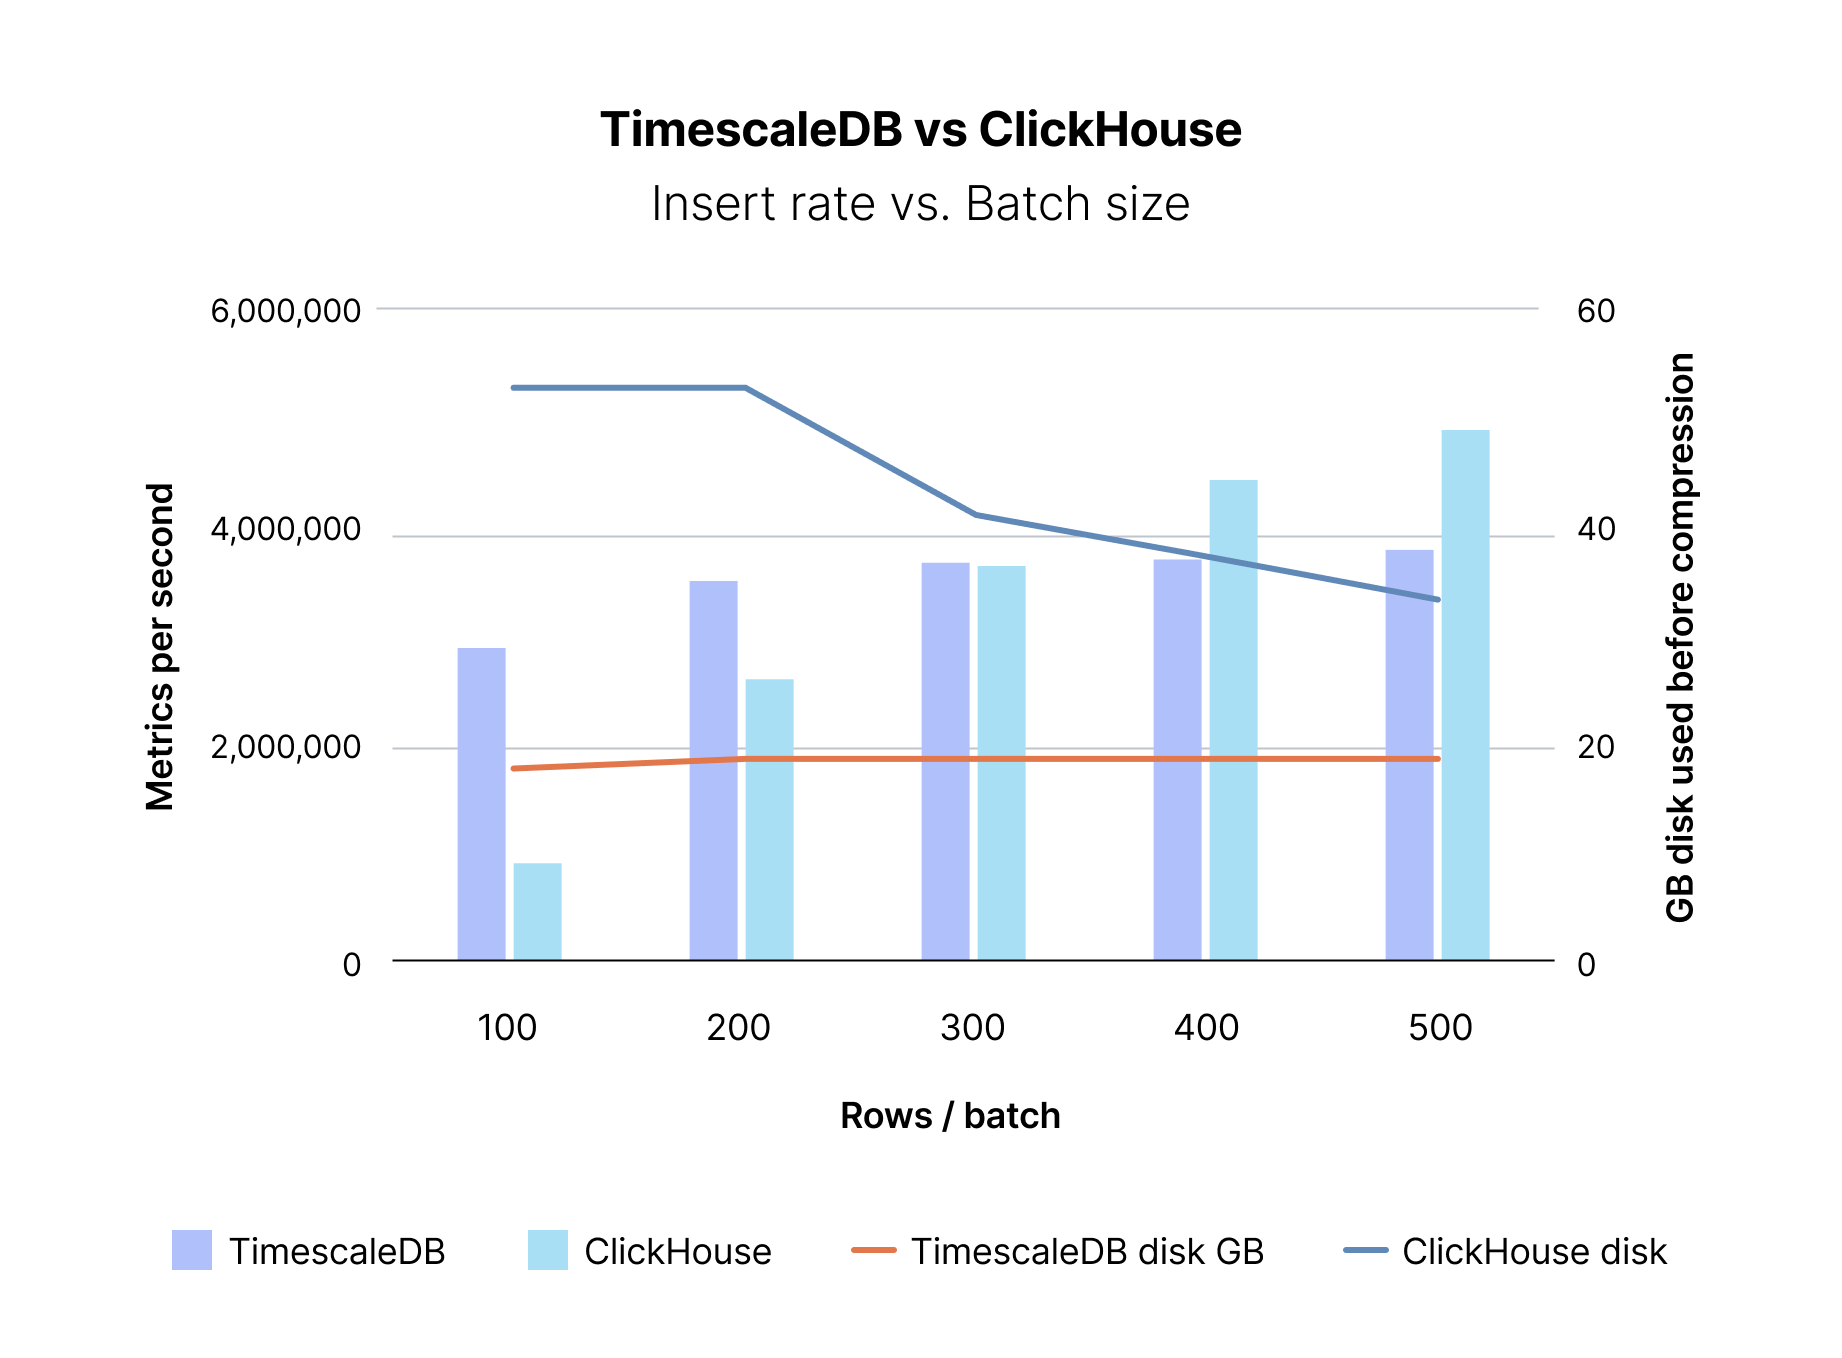
\includegraphics[width=0.85\textwidth]{imgs/02-small-batch-insert-performance.png}
	\captionof{figure}{\href{https://www.timescale.com/blog/what-is-clickhouse-how-does-it-compare-to-postgresql-and-timescaledb-and-how-does-it-perform-for-time-series-data/}{Timescale ha performance migliori di \href{https://7last.github.io/docs/pb/documentazione-interna/glossario\#clickhouse}{ClickHouse\textsubscript{G}} con batch di dimensione più contenuta e usa una quantità di disco inferiore di 2.7 volte}}
\end{center}

\begin{center}
	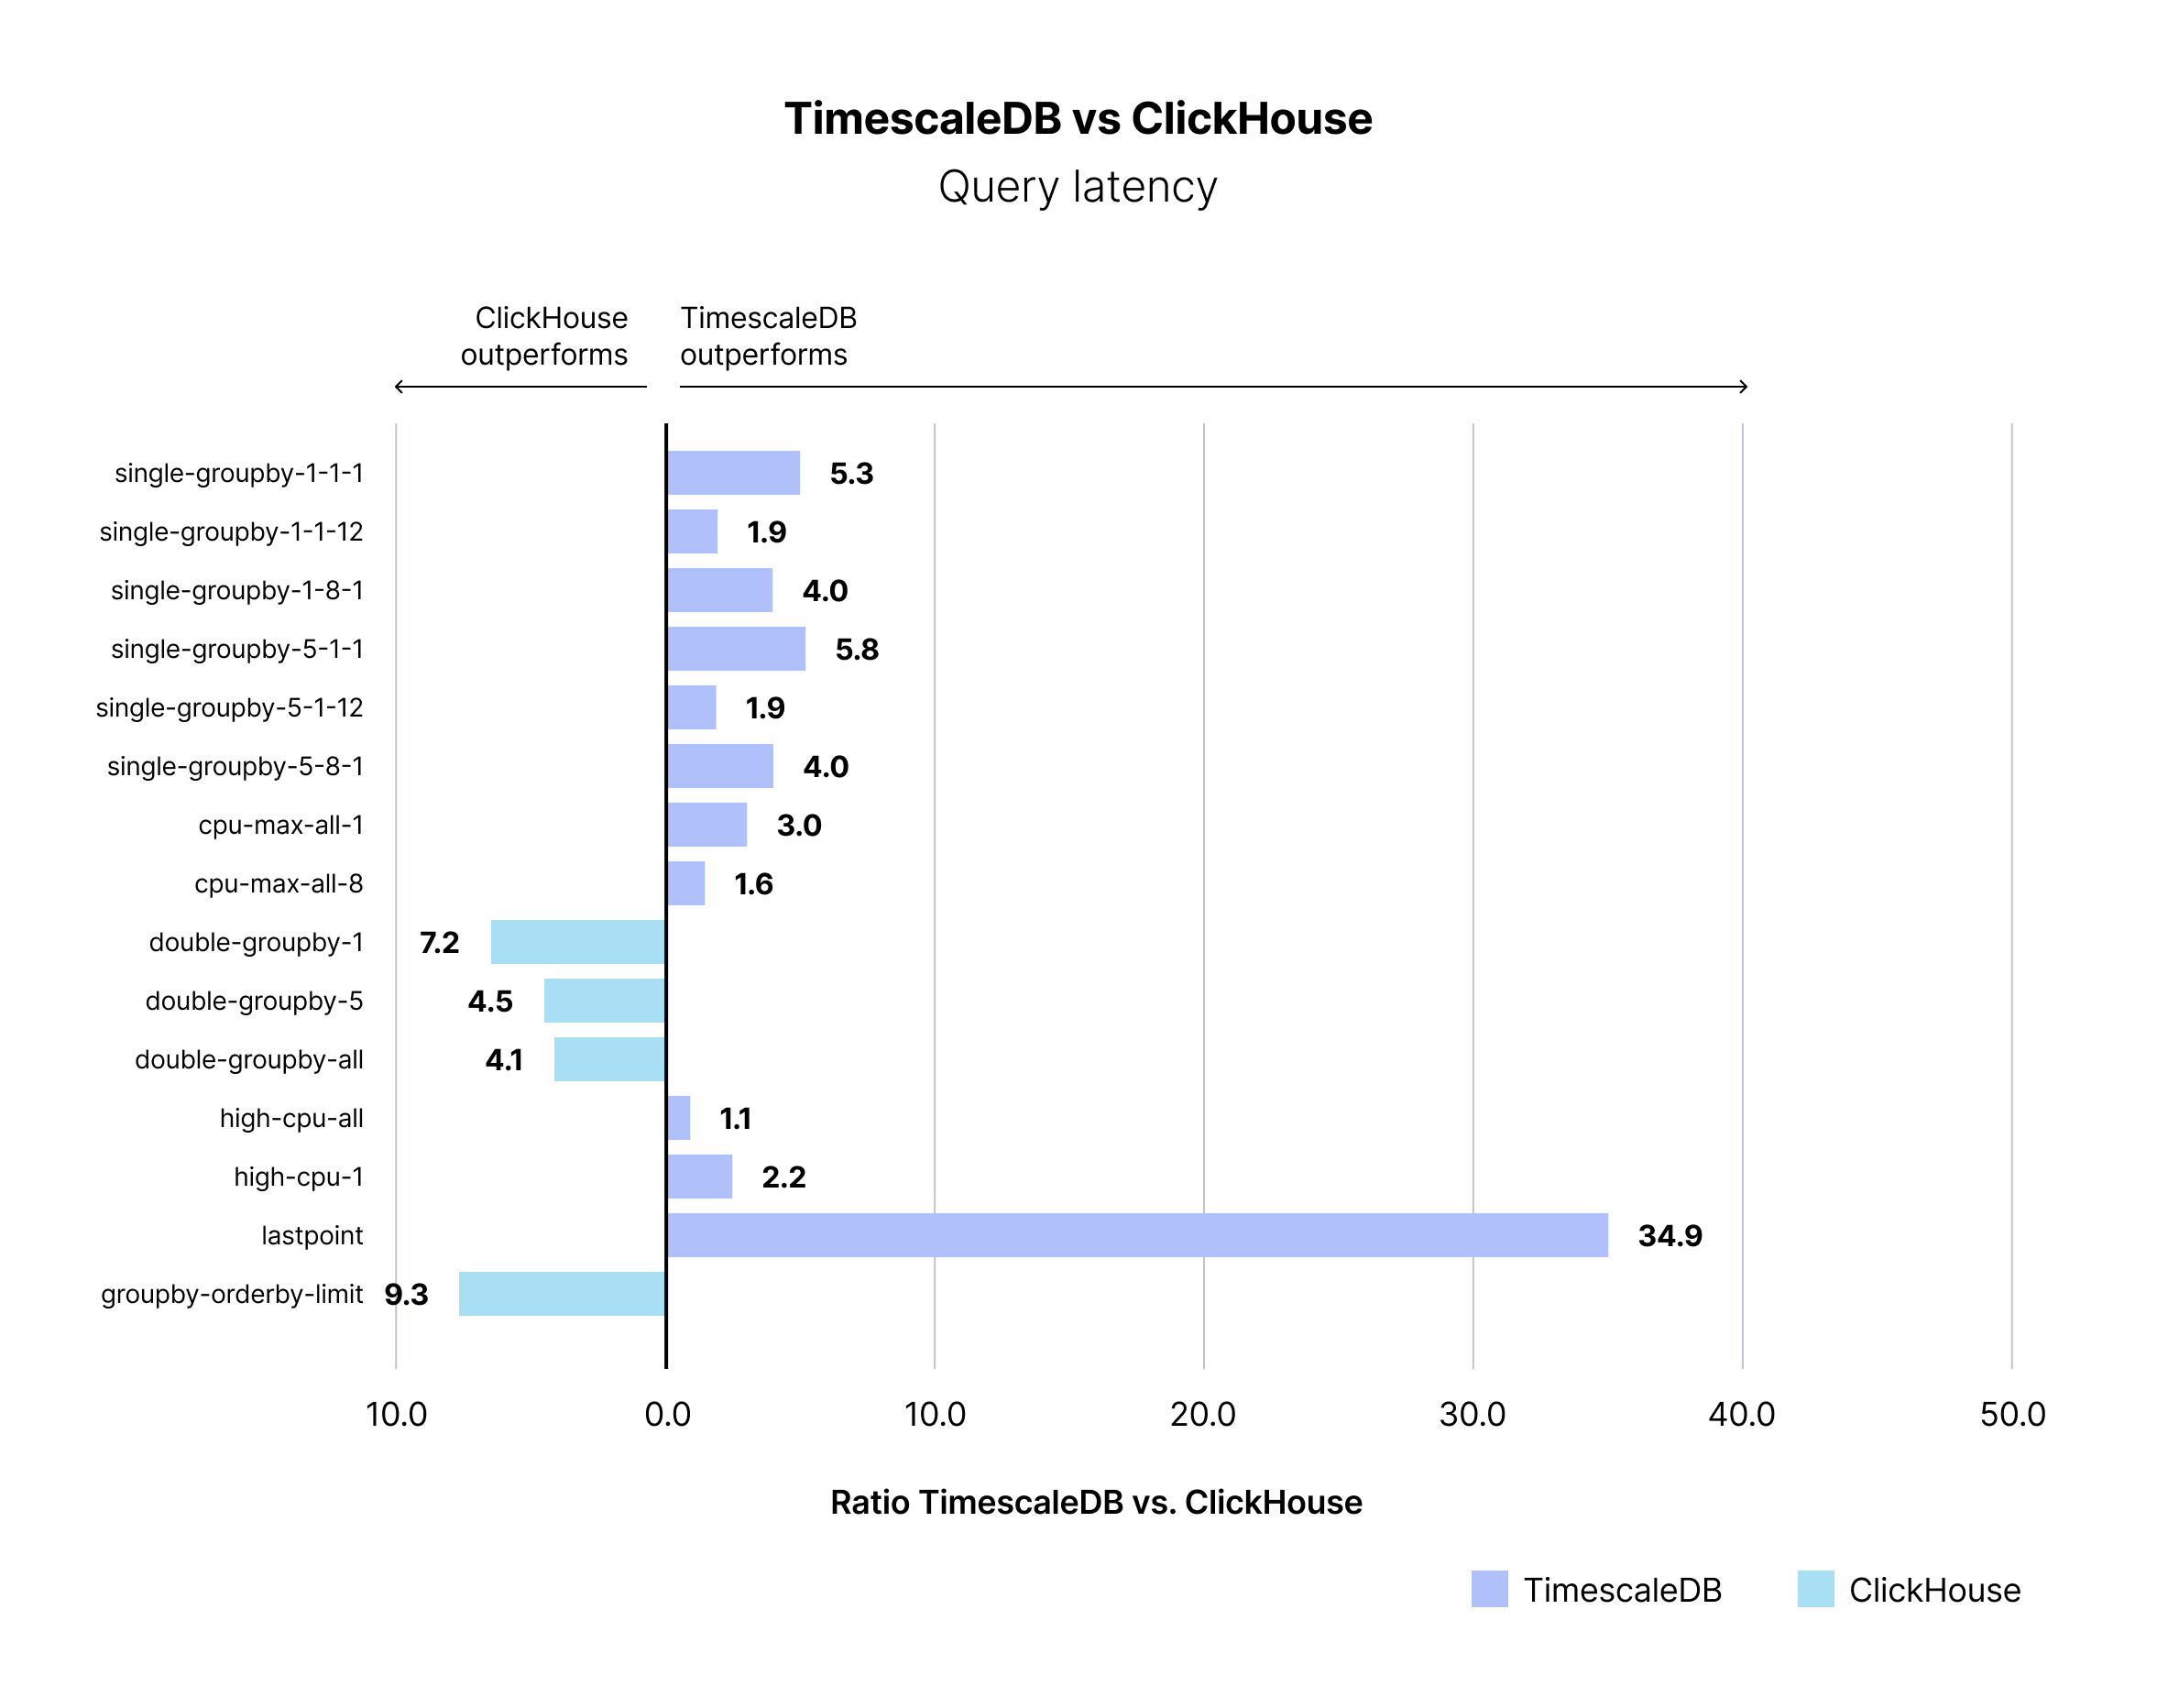
\includegraphics[width=0.85\textwidth]{imgs/03-query-latency.png}
	\captionof{figure}{\href{https://www.timescale.com/blog/what-is-clickhouse-how-does-it-compare-to-postgresql-and-timescaledb-and-how-does-it-perform-for-time-series-data/}{Performance relative alle query}}
\end{center}

\begin{center}
	\includegraphics[width=0.85\textwidth]{imgs/07-\href{https://7last.github.io/docs/pb/documentazione-interna/glossario\#clickhouse}{clickhouse\textsubscript{G}}-improvement.png}
	\captionof{figure}{\href{https://www.timescale.com/blog/what-is-clickhouse-how-does-it-compare-to-postgresql-and-timescaledb-and-how-does-it-perform-for-time-series-data/}{Performance degli insert}}
\end{center}

\begin{center}
	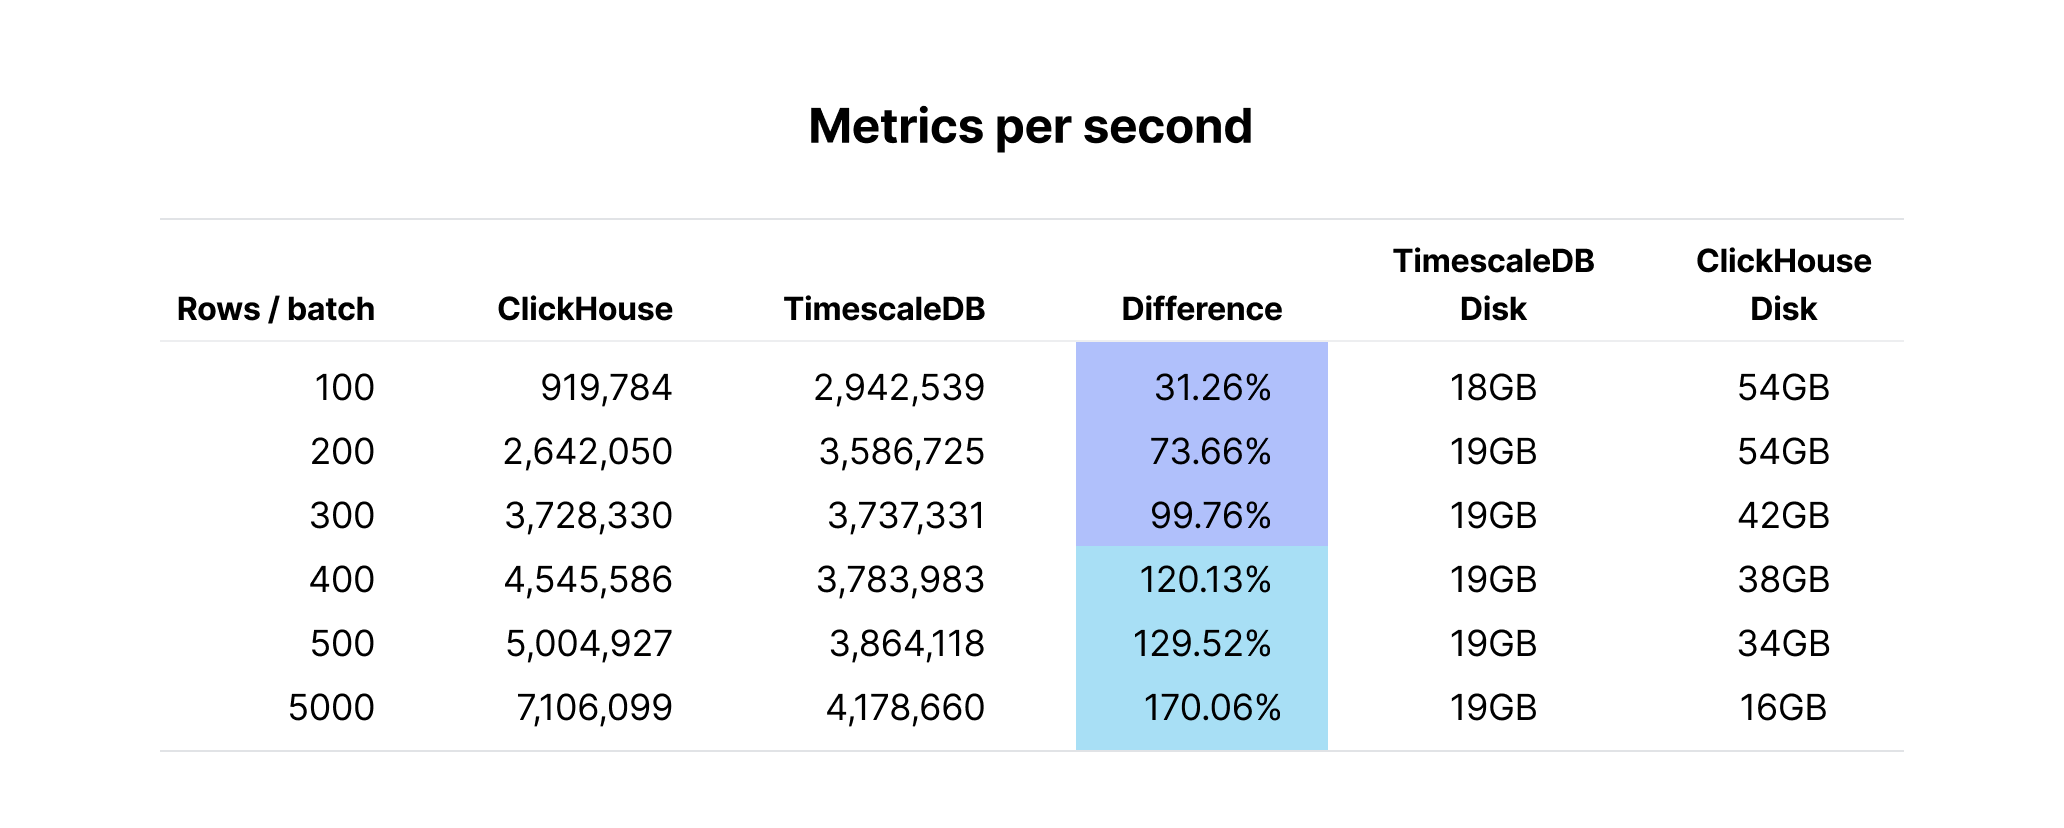
\includegraphics[width=0.85\textwidth]{imgs/08-chunk-time-interval.png}
	\captionof{figure}{\href{https://www.timescale.com/blog/what-is-clickhouse-how-does-it-compare-to-postgresql-and-timescaledb-and-how-does-it-perform-for-time-series-data/}{Performance degli insert con batch di dimensioni ridotte}}
\end{center}

\begin{center}
	\includegraphics[width=0.85\textwidth]{imgs/09-\href{https://7last.github.io/docs/pb/documentazione-interna/glossario\#clickhouse}{clickhouse\textsubscript{G}}-benchmark-read-latency-performance.png}
	\captionof{figure}{\href{https://www.timescale.com/blog/what-is-clickhouse-how-does-it-compare-to-postgresql-and-timescaledb-and-how-does-it-perform-for-time-series-data/}{Performance di query di 4000 host con 100 milioni di righe di dati}}
\end{center}

\begin{center}
	\includegraphics[width=0.85\textwidth]{imgs/10-\href{https://7last.github.io/docs/pb/documentazione-interna/glossario\#clickhouse}{clickhouse\textsubscript{G}}-benchmark-read-latency-performance.png}
	\captionof{figure}{\href{https://www.timescale.com/blog/what-is-clickhouse-how-does-it-compare-to-postgresql-and-timescaledb-and-how-does-it-perform-for-time-series-data/}{Performance di query di 10000 host con 100 milioni di righe di dati}}
\end{center}








\section{Conclusioni}
Se sono necessarie query su dataset ampi e poco mutevoli, eseguite da pochi utenti Clickhouse è la scelta adatta.
Se invece sono presenti casi d’uso tipici di un database OLTP ed è necessaria l'implementazione di time-series TimescaleDB è la soluzione.
Nel nostro caso gli ambiti di utilizzo rispecchiano pienamente quelli di ClickHouse.







\end{document}



